% !TeX spellcheck = fr_FR
\chapter{Chapitre 1 : Analyse}

Ce chapitre a pour but d'expliquer de manière détaillée l'objectif de ce projet de semestre. Je vais aussi faire part des différentes idées qui sont ressorties lors de nos discussions avec mon professeur. Par la suite, je vais expliquer en quoi consiste la fonction de hachage Bcrypt, son fonctionnement et ses spécificités. Pour finir, je vais rapporter les différentes implémentations sur \gls{fpga} que j'ai pu retrouver et celui que j'ai fini par reprendre durant le projet de semestre. 

\section{Description du projet}

L'objectif principal de ce projet est d'exploiter le parallélisme offert par les \gls{fpga}, afin de calculer les fonctions de hachage nécessitant beaucoup de temps de calculs. Le but étant d'avoir au final un système plus efficient que les solutions actuelles lors d'une attaque par bruteforce. Il est aussi nécessaire d'avoir une certaine communication entre le \gls{pc} de l'attaquant et le \gls{fpga}, afin que l'attaquant puisse fournir le hash qu'il souhaite casser.

\begin{figure}[tbph!]
	\centering
	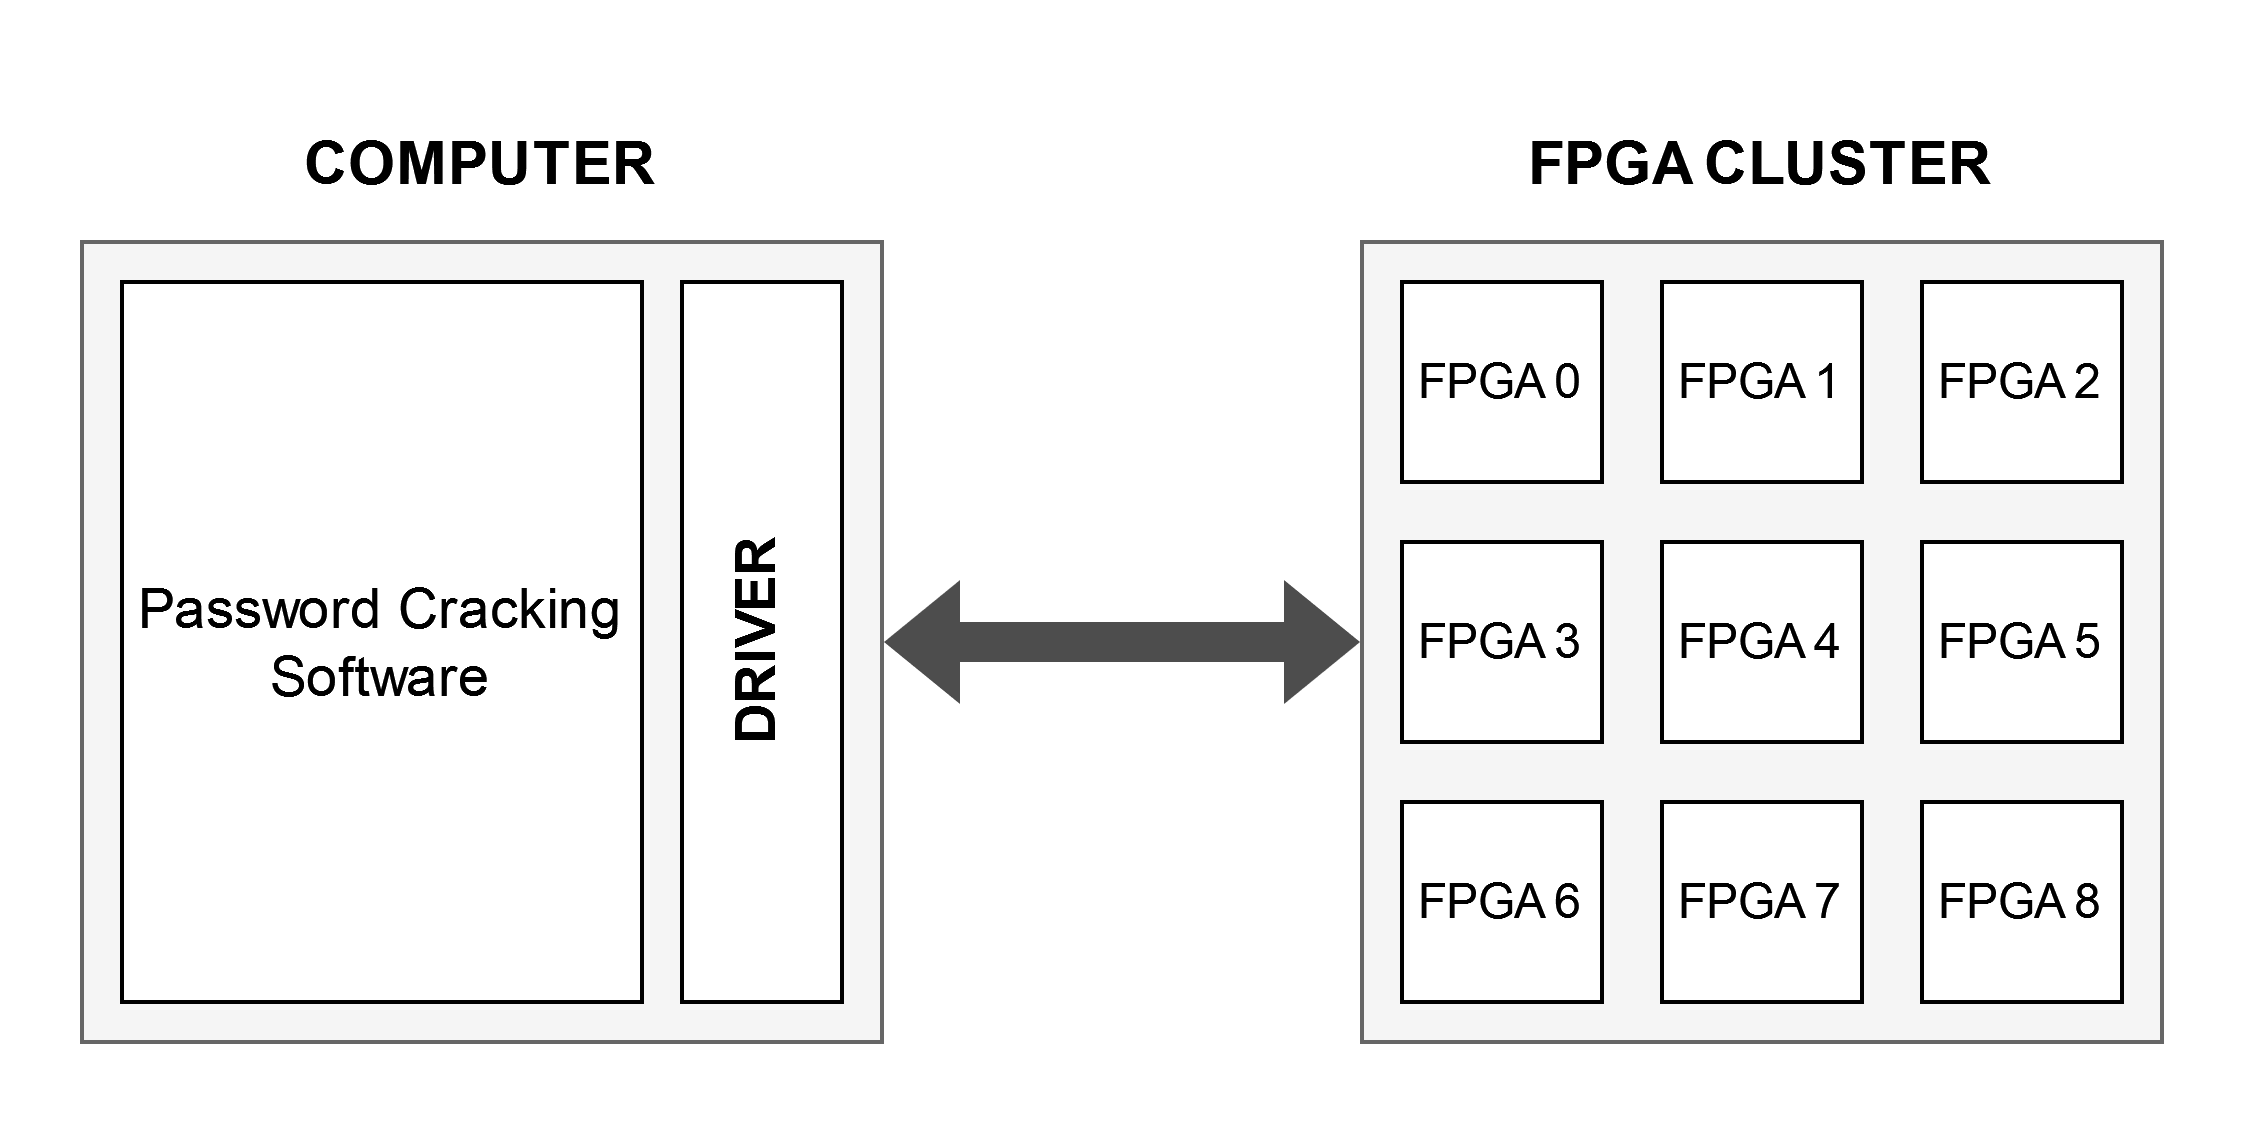
\includegraphics[width=0.7\linewidth]{objectif}
	\caption[Diagramme général]{Diagramme général. Source : réalisé par Kandiah Abivarman}
	\label{fig:objectif}
\end{figure}

Une des première question qu'on s'était posée avec les professeurs était la manière pour générer les mots de passe lors d'une attaque. Dans notre cas, nous avons deux possibilités, soit nous générons les mots de passe directement depuis le \gls{pc} et devons les transmettre à la carte \gls{fpga} afin de procéder au hachage, sinon la génération se fait directement dans le \gls{fpga}. La différence est que dans le premier cas, on peut être possiblement limité au niveau logiciel par le \gls{pc} ou au niveau de la communication avec le \gls{fpga}. Toutefois, au niveau de la génération des mots de passe on aura plus de flexibilité permettant d'autres types d'attaques comme par exemple une attaque par dictionnaire\footnote{TO DO}.

Pour le projet de semestre, j'ai décidé de partir plutôt vers la génération sur \gls{fpga}, afin d'avoir une première solution entièrement fonctionnelle sur \gls{fpga} sans dépendance avec un \gls{pc}. La génération sur \gls{pc} est toutefois envisageable par la suite pour le projet de bachelor.

\section{Bcrypt}



\subsection{Algorithme}



\subsection{Format du Hash}


\section{Implémentations Existantes}